%File: formatting-instruction.tex
\documentclass[letterpaper]{article}
\usepackage{aaai}
\usepackage{times}
\usepackage{helvet}
\usepackage{courier}
\usepackage[utf8]{inputenc}
\usepackage[english]{babel}
\usepackage{amsmath}
\usepackage{amssymb}
\usepackage{amsthm}
\usepackage{color}
\usepackage[ruled, vlined,linesnumbered]{algorithm2e}
\usepackage{graphicx}
\newtheorem{theorem}{Theorem}
\newtheorem{lemma}{Lemma}
\newtheorem{proposition}{Proposition}
\newtheorem{corollary}{Corollary}
\usepackage{color}
\theoremstyle{definition}
\newtheorem{definition}{Definition}

\usepackage{subcaption}
\newcommand{\zherong}[1]{\textcolor{blue}{#1}}
\newenvironment{zherongBlk}{\color{blue}}{}

% ------------------------------------------------------------------------theorem
\makeatletter
\def\thm@space@setup{%
  \thm@preskip=\parskip \thm@postskip=0pt
}
\makeatother
\theoremstyle{plain}
\newtheorem{thm}{Theorem}[section]
\newtheorem{lem}[thm]{Lemma}
\newtheorem{prop}[thm]{Proposition}
\newtheorem*{cor}{Corollary}

\theoremstyle{definition}
\newtheorem{defn}{Definition}[section]
\newtheorem*{defn*}{Definition}
\newtheorem{conj}{Conjecture}[section]
\newtheorem{exmp}{Example}[section]

\theoremstyle{remark}
\newtheorem*{rem}{Remark}
\newtheorem*{note}{Note}
% ------------------------------------------------------------------------

\frenchspacing
\setlength{\pdfpagewidth}{8.5in}
\setlength{\pdfpageheight}{11in}
\pdfinfo{
/Title ()
/Author ()}
\setcounter{secnumdepth}{0}  
 \begin{document}
% The file aaai.sty is the style file for AAAI Press 
% proceedings, working notes, and technical reports.
%
\title{Supplemental Document of Paper 1159}
\author{Paper ID: 2911}
\maketitle
\begin{theorem}
For an agent, if it does not overlap with any obstacle, there will be at least one circle $A(\mathbf v,ran)$ existing which includes this agent. That is, $\{\mathbf{a} | \mathbf{a} \cap \mathcal{O} = \varnothing, \exists{ A(\mathbf v,ran)}, \mathbf{a} \subseteq  A(\mathbf v,ran)\}$
\label{thm:included}
\end{theorem}


\begin{figure}[!ht]
\centering
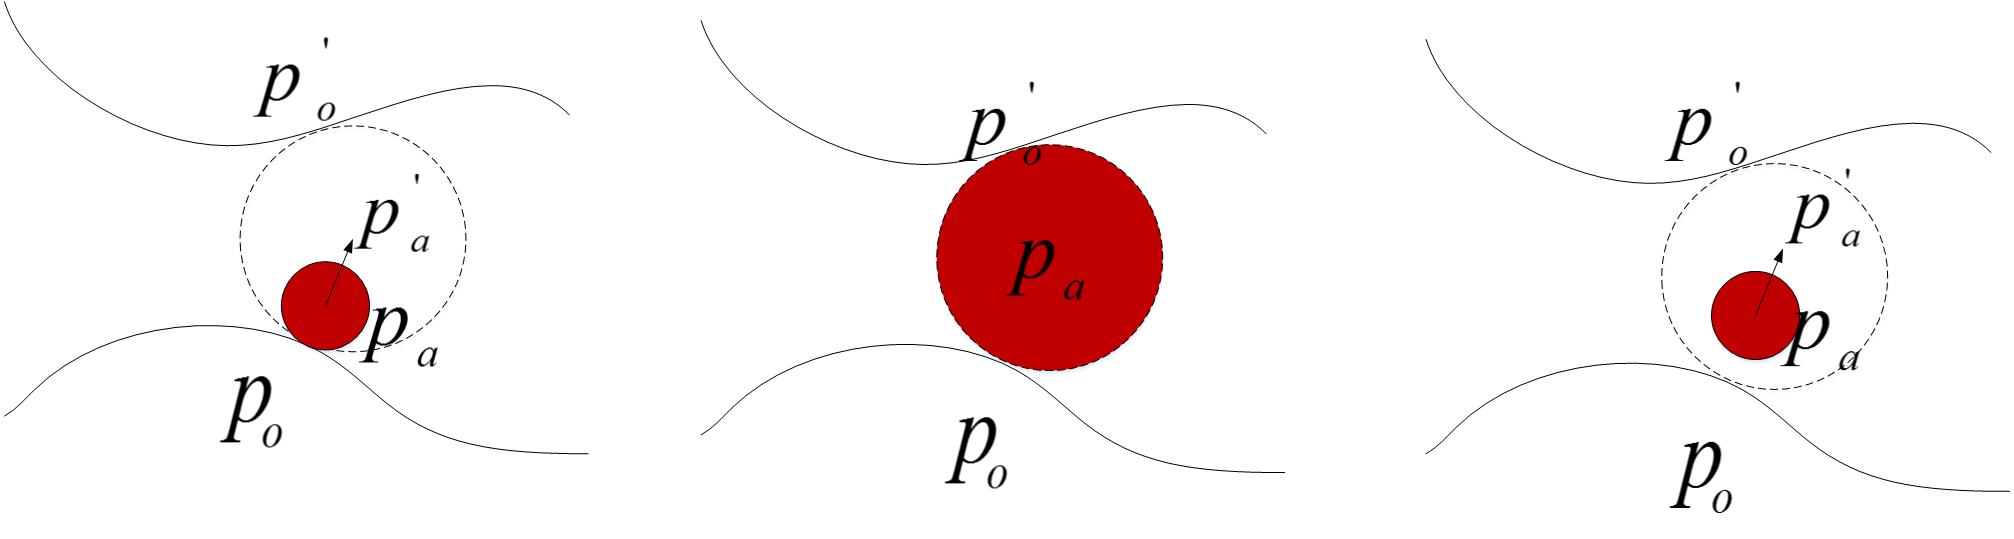
\includegraphics[width=1\linewidth]{figs/include.png}
\caption{This figure shows the three scenarios that are shown in the proof of theorem \ref{thm:included}. In the left figure, the agent (red) is a tangent to the obstacles at a single point. The dot-line circle represents the expanded circle which is illustrated in the proof of theorem \ref{thm:included}.
In the center figure, the agent is tangent to the obstacles at two different points and it overlaps with the corresponding circle. In the right figure, the agent is not tangent to any point of the obstacles.
}
\label{fig:include}
\end{figure}
\begin{proof}
The proof of Theorem \ref{thm:included} is based on three different scenarios. We illustrate these situations in Figure \ref{fig:include}.
We first consider the scenario in which the agent $a$  is only tangent to the edge of obstacles $\mathcal{O}$ at one point. In this case, we incrementally move the position of the agent $\mathbf p_a$ along
the direction $\mathbf p_a- \mathbf p_o$ and note the new position as $\mathbf p'_a$. 
Meanwhile, we create a circle $A(\mathbf p'_a,\|\mathbf p_o- \mathbf p'_a\|)$ where the $\mathbf p_o$ is the tangent point between the circle and the obstacle. We can observe that $\mathbf a \subseteq A(\mathbf p'_a,\|\mathbf p_o- \mathbf p'_a\|)$. $\mathbf p'_a$ keeps moving away from $\mathbf p_o$ and $A(\mathbf p'_a,\|\mathbf p_o- \mathbf p'_a\|)$ is enlarging while $A(\mathbf p'_a,\|\mathbf p_o- \mathbf p'_a\|)$ touches $\mathcal{O} $ at $\mathbf p_o$ all the time. 
When $A(\mathbf p'_a,\|\mathbf p_o- \mathbf p'_a\|)$ touches more than one point of $\mathcal{O}$, the enlarging will stop. According to the definition of the medial-axis, $A(\mathbf v,\|\mathbf p_o- \mathbf p'_a\|)$ has to be a valid circle of $\mathcal G$.
 %%%%%%%%%%%%%%situation 1 
In the second scenario, suppose $\mathbf a$ touches more than one point of $\mathcal{O}$. According to the definition of the medial-axis $\mathbf a$ is overlapping with a corresponding circle.
In the third scenario, assuming $\mathbf a$ does not touch any part of $\mathcal{O}$, we expand the radius of agent $r'$ until the new circle $A(\mathbf p_a, r')$ touches one or more points of $\mathcal{O}$. Then this situation can transition to one of the above situations. By now, we have proved Theorem \ref{thm:included}. 
\label{proof:included}
\end{proof}




\begin{lemma}
Assume a cluster $\mathbf{A}$ and its incident circle $A(\mathbf v,ran)$ is non-full, $\forall \mathbf{a} \in \mathbf{A}$. We can find a complete path from its start position $\mathbf{p_a} \in A(\mathbf v,ran)$ to the goal position $\mathbf{p_a'} \in A(\mathbf v,ran)$ and we then call $\mathbf{A}$ complete. 
\label{lem:intra-unit complete}
\end{lemma}
\begin{proof}
We use Algorithm \ref{algo:intramovement} to move the agents to their goals, which are inside of $A(\mathbf v,ran)$. Before running the algorithm, we assume the agents have already been arranged in a circular pattern.
Algorithm \ref{algo:intramovement} repeatedly uses the intra-loop and inter-loop to move the elements to their goals. Since $A(\mathbf v,ran)$ is non-full, it must at least have an empty element so both the intra-loop and inter-loop are executable. We then prove Lemma \ref{lem:intra-unit complete}.
\label{proof:intra-unit complete}
\end{proof}

\begin{figure}[!ht]
\centering
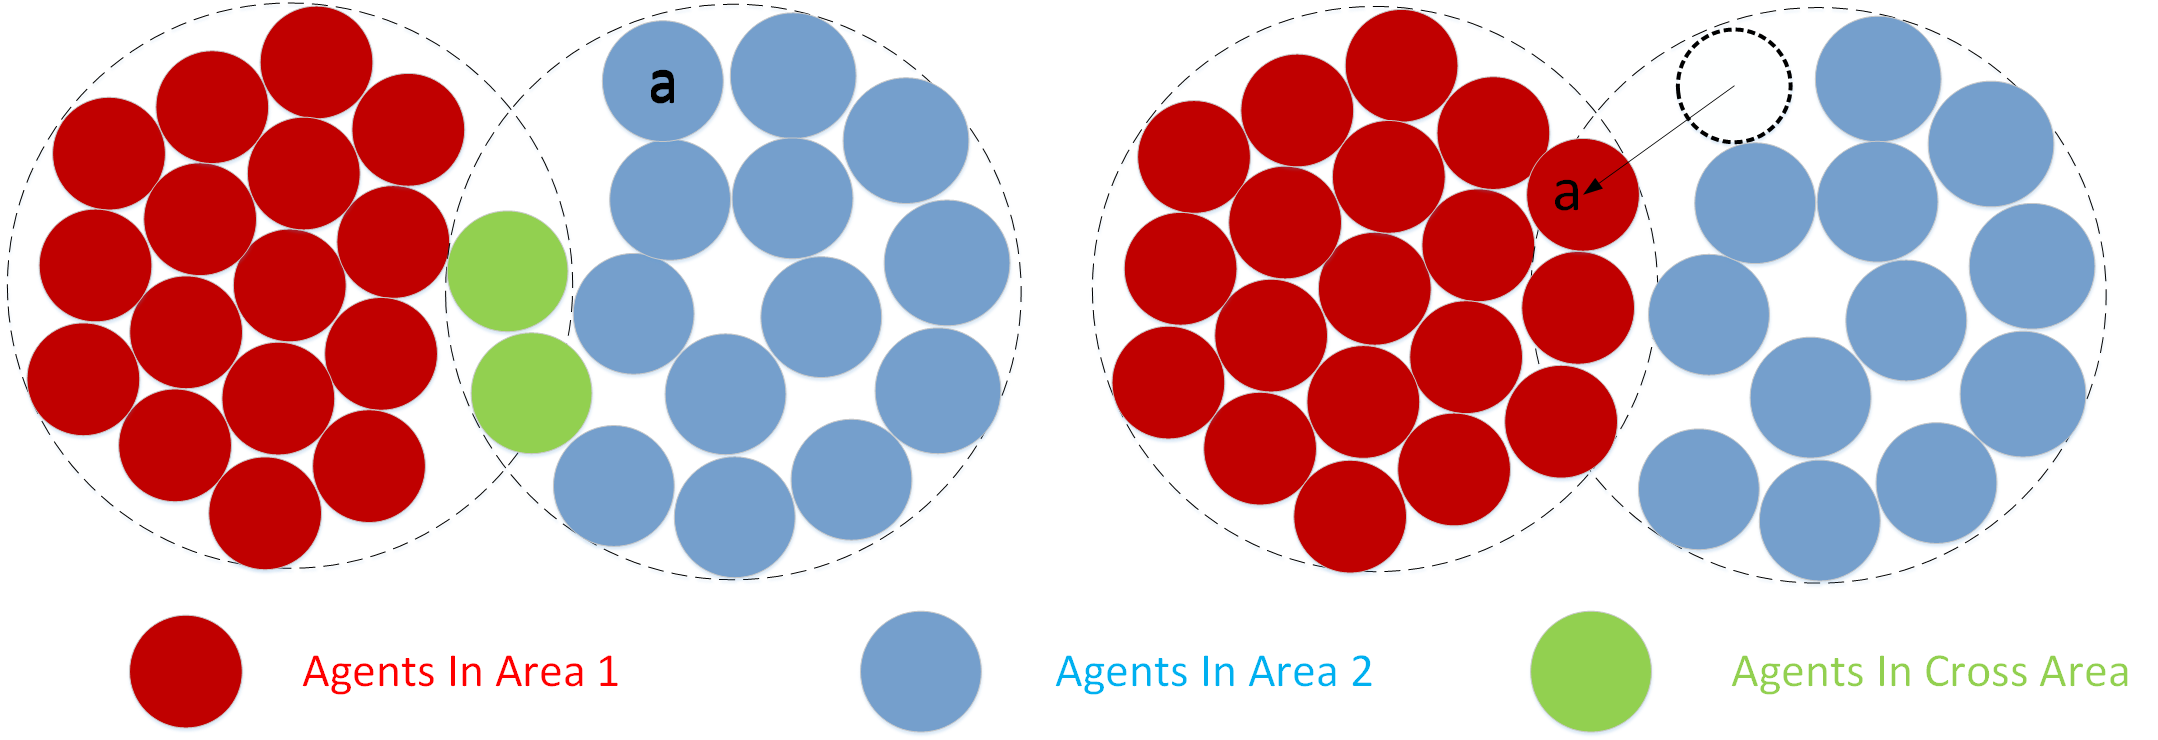
\includegraphics[width=1\linewidth]{figs/ConnectClusters.png}
\caption{
In this figure, we show how to check whether or not the combined area of two circles is full. In the left picture, two circular areas are filled with several agents. Notice the green disc-like agents landing in the crossed area of the two circles. In the right picture, to fill the left circular area to a tight arrangement, it needs to move one more agent from the right area $a$. It turns out that the right circle is not full. 
}
\label{fig:combinedcircles}
\end{figure}
As we introduced in a previous section, the circle packing is a problem, because the combined area is no longer a circle when several circular areas cross each other. It is therefore difficult to use the algorithm ~\cite{graham1998dense} to analyze whether the area is full or not. Here we first introduce a simplified method to check if two combined circular areas are full or not. Multiple circles' situation can then be deduced from the result.
Assume two clusters $\mathbf{A}$ and $\mathbf{A'}$ with their two circular areas $A(\mathbf v,ran) \cap A(\mathbf v',ran') \neq \varnothing$. We classify the agents in this combined area into three categories: $\mathbf{A_0} \subset A(\mathbf v,ran)$, $\mathbf{A_1} \cap (A(\mathbf v,ran) \cap A(\mathbf v',ran') ) \neq \varnothing$ and $\mathbf{A_2} \subset A(\mathbf v',ran')$, shown in Figure
\ref{fig:combinedcircles} as red, green and blue respectively. We complete the following movement to check if this combined area is full; first try to fill one of area let's say $A(\mathbf v,ran)$ to tight arrangement, if $A(\mathbf v,ran)$ has one more agent which was belonged to $\mathbf{A_2}$ then the combined area is non-full. If not, we then try to fill  $A(\mathbf v',ran')$ to tight arrangement to see if it includes an agent that belonged to $\mathbf{A_0}$. If it does, then the combined area is non-full, otherwise, we claim the combined area is full. Figure \ref{fig:combinedcircles} shows one such this processing.
For all of clusters if their incident circular areas cross each other, then we can use the above method to check if they are full or not, and treat them as an united cluster. 

\begin{lemma}
If two areas $A(\mathbf v, ran)$ and $A(\mathbf v', ran')$ are connected, and at least one of them is non-full, then all of their elements can reach any position if $\{\mathbf{p}| \mathbf{p} \in A(\mathbf v, ran) \cup A(\mathbf v', ran')\}$ .
\label{lem:intertcluster}
\end{lemma}
\begin{proof}
In this proof, we only discuss the situation that one of the areas is full. The situation of two non-full areas whose proof can be deducted from this one.

Suppose one of the areas $A(\mathbf v,ran)$ is non-full and the other $A(\mathbf v',ran')$ is full. We divide all of the element's movement into four situations. 
For the first situation, assume $\mathbf{c} \subseteq A(\mathbf v,ran)$ and that the goal of $\mathbf{c}$ is $\mathbf{p_c} \in A(\mathbf v,ran)$. This situation has already been proved by Lemma \ref{lem:intra-unit complete}.
For the second situation, assume $\mathbf{c} \subseteq A(\mathbf v,ran)$ and that the goal of $\mathbf{c}$ is $\mathbf{p_c} \in A(\mathbf v',ran')$.
We can decompose this situation into three steps. For the first step, move $\mathbf{c}$ and empty element $\mathbf{e}$ to the outer-most loop of  $A(\mathbf v,ran)$. In the next step, move a $\mathbf{c'} \subseteq A(\mathbf v',ran')$ to $\mathbf{p_e}$. Note that now $A(\mathbf v',ran')$ is non-full. For the last step, move $\mathbf{c}$ to $A(\mathbf v',ran')$, and $A(\mathbf v',ran')$ is full again. Finally, move $\mathbf{c''} \subseteq A(\mathbf v',ran')$ to $A(\mathbf v,ran)$. Then  $\mathbf{c} \subseteq A(\mathbf v',ran')$ and $\mathbf{p_c} \in A(\mathbf v',ran')$ ,so we transition this situation to first situation. 
For the third situation, assume $\mathbf{c} \subseteq A(\mathbf v',ran')$ and the goal of $\mathbf{c}$ is $\mathbf{p_c} \subseteq A(\mathbf v',ran')$. We can move another element $\mathbf{c'} \subseteq A(\mathbf v',ran')$ to transition this situation to the first situation.
For the fourth situation, assume $\mathbf{c} \subseteq A(\mathbf v',ran')$ and the goal of $\mathbf{c}$ is $\mathbf{p_c} \subseteq A(\mathbf v,ran)$. We move another element $\mathbf{c'} \subseteq A(\mathbf v',ran')$ to $A(\mathbf v',ran')$, and then this situation has been changed into the second situation. Then we prove the Lemma \ref{lem:intertcluster}.
\label{proof:intertcluster}
\end{proof}

\begin{lemma}
Suppose all clusters are connected. If there is one of cluster whose area is not full, or we can remove an agent from a full area to a new place without impacting the clearance of all the paths between clusters, then we can find a solution to move all agents to their goal. Otherwise, there is no solution for the current scenario.
\label{lem:complete}
\end{lemma}

\begin{proof}
Suppose we have a clean path and there are sequential agents' clusters with their area $ A^0(\mathbf v,ran), A^1(\mathbf v,ran),... A^n(\mathbf v,ran)$ on this path. We have an agent $\mathbf{a} \subset A^0(\mathbf v,ran)$ and its goal $\mathbf{p} \in A^n(\mathbf v,ran)$. Assume one agent of area $ A^t(\mathbf v,ran)$ is not full and has an empty element $\mathbf{e} \subset A^t(\mathbf v,ran)$. We can then perform the following movements to move $\mathbf{a}$ to $A^n(\mathbf v,ran)$. First, move $\mathbf{e}$ to $A^1(\mathbf v,ran)$. According to Lemma ~\ref{lem:intertcluster}, $\mathbf{a}$ can be moved to $A^n(\mathbf v,ran)$. Repeatedly move $\mathbf{e}$ with $\mathbf{a}$ to $A^n(\mathbf v,ran)$, and then use the intra-loop and inter-loop exchange algorithm to move $\mathbf{a}$ to $\mathbf{p}$. We thus prove Lemma ~\ref{lem:complete}.
\label{proof:complete}
\end{proof}
\begin{algorithm}[!th]
  \SetKwInOut{Input}{input}\SetKwInOut{Output}{output}
  \Input{An element $\mathbf{c}$ in a loop $\mathbf{T}$ and another element $\mathbf{c'}$ in another loop $\mathbf{T'}$.}
  \Output{$\mathbf{c}$ and $\mathbf{c'}$ exchange their positions, while the rest of elements of $A$ do not change their positions.}
  \BlankLine
  \If{$A$ is non-full}{
  \If{$\mathbf{c}$ is not connected with any empty element $\mathbf{e} \in \mathbf{T} $}{
    Exchange an empty element $\mathbf{e} \in A$ with an element $\mathbf{c_n}$, $\mathbf{c_n} \in \mathbf{T}$ and $\mathbf{c_n} \sim \mathbf{c}$.\\
    }
    \While{ $|\mathbf{T} - \mathbf{T'}| \neq 0$ }{
   Keep running Neighboring Loops Exchange to move $\mathbf{c}$ and $\mathbf{e}$ toward the loop of $\mathbf{c'}$
  }
   Run Intra-loop exchange to exchange $\mathbf{c'}$ and $\mathbf{c}$\\
   Move $\mathbf{e}$ with $\mathbf{c'}$ to $\mathbf{T}$ while return all moved elements to their primitive positions.\\
   Run Intra-loop algorithm to move $\mathbf{c}$ to $\mathbf{p_c'}$\\
   \If{$\mathbf{e}$ moved from other position}{
        Return $\mathbf{e}$ to its primitive position 
   }
  }
  
  \Else{
  \tcc{otherwise, the solution does not exist.}
    \Return FALSE
  }
  \caption{Inter-loop Exchange: This is used in Algorithm 2, Step 7 and 8.}
  \label{algo:interloop}
\end{algorithm}
\begin{quote}
\begin{small}
\bibliographystyle{aaai}
\bibliography{reference}
\end{small}
\end{quote}





%\section{ Acknowledgments}

%\bigskip
%\noindent Thank you for reading these instructions carefully. We look forward to receiving your electronic files!

\end{document}
